\documentclass[8pt]{beamer}
\usepackage[T1]{fontenc}
\usepackage[utf8]{inputenc}
\usepackage[polish]{babel}
\usepackage{amsfonts}
\usepackage{amssymb}
\usepackage{amsthm}
\usepackage{amsmath} 
\usepackage{color}
\usepackage{times}

%\usetheme{Warsaw}
%\usetheme{Madrid}
%\usetheme{AnnArbor}
%\usetheme{Rochester}
%\usetheme{Boadilla}
%---------------------------------------------------------------------------
\usetheme{default}

\begin{document}
\usebackgroundtemplate{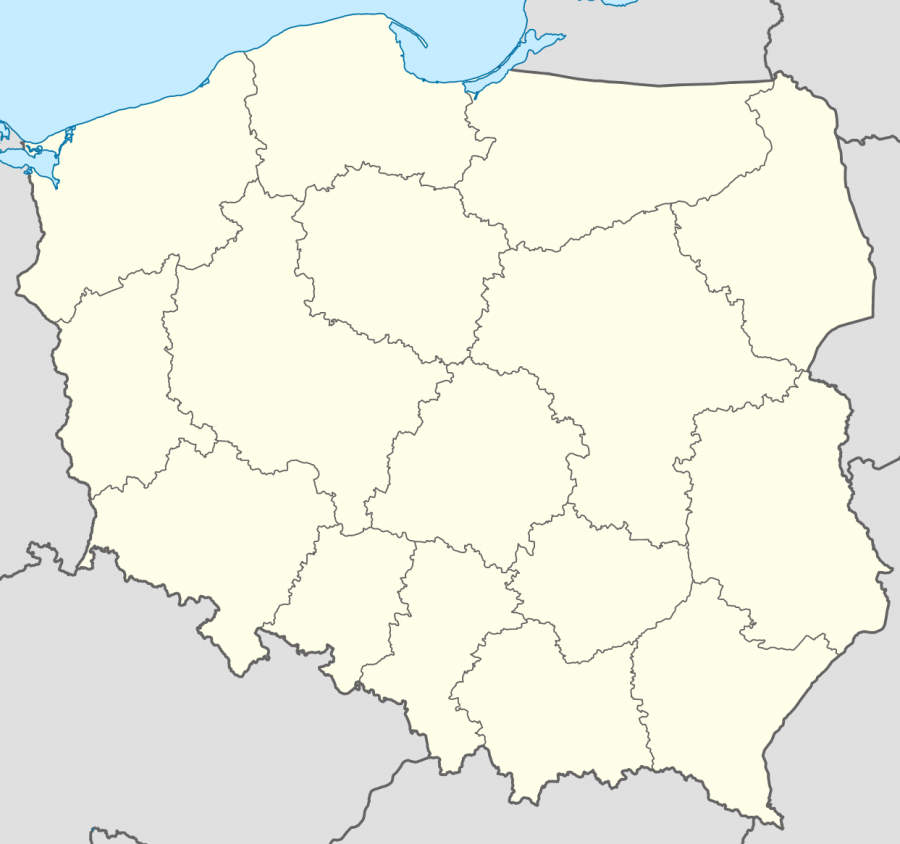
\includegraphics[width=\paperwidth,height=\textheight]{Polska}}

\begin{frame}[t]
\frametitle{Alfabet, słowo, słownik} 
\begin{columns}
	\column{0.6\textwidth}
\begin{alertblock}{}
\alert{Alfabetem} nazywamy dowolny skończony zbiór $\Sigma$.
\end{alertblock}

\begin{exampleblock}{}
$\Sigma = \{a,b,\dots,z,A,B,\dots,Z\}$ -- alfabet łaciński\\
$\Sigma = \{\alpha,\beta,\dots,\omega\}$ -- alfabet grecki (małe litery)\\
$\Sigma = \{0,1\}$ -- alfabet binarny\\
$\Sigma = \{\cdot,-\}$ -- alfabet Morse'a
\end{exampleblock}
\column{0.35\textwidth}
\end{columns}
\pause
\begin{columns}
\column{0.35\textwidth}
\column{0.6\textwidth}
\begin{alertblock}{}
\alert{Słowem} w alfabecie $\Sigma$ nazywamy dowolny skończony ciąg liter alfabetu $\Sigma$ oraz \alert{słowo puste} $\varepsilon$. 

\alert{Słownikiem nad alfabetem} $\Sigma$ nazywamy zbiór wszystkich słów nad alfabetem $\Sigma$ i~oznaczamy symbolem $\Sigma^{*}$. Przyjmiemy ponadto oznaczenie: $\Sigma^{+} = \Sigma^{*} - \{\varepsilon\}$.
\end{alertblock}

\begin{exampleblock}{}
$\Sigma = \{0,1,2,\dots,9\}$, Przykłady słów: $\varepsilon$, 0, 1, 7, 56, 123, 007, 00000,\,\dots
\end{exampleblock}

\end{columns}

\end{frame}

%---------------------------------------------------------------------------

\begin{frame}[t]
\frametitle{Słowo, długość słowa} 
\begin{columns}
	\column{0.35\textwidth}
\begin{alertblock}{rekurencyjna definicja słowa nad alfabetem $\Sigma$}
\begin{enumerate}
\item $\varepsilon$ jest słowem nad alfabetem $\Sigma$; 
\item jeśli $x$ jest słowem nad alfabetem $\Sigma$ i~$a \in \Sigma$, to $xa$ jest słowem nad alfabetem $\Sigma$;
\item nic innego nie jest słowem nad alfabetem $\Sigma$ poza tym, co wynika z (1) i~(2).
\end{enumerate}
\end{alertblock}
\column{0.35\textwidth}
\pause

\begin{alertblock}{}
Ilość liter w słowie $x$ nazywamy \alert{długością słowa} $x$ i oznaczamy symbolem $|x|$. Przyjmujemy ponadto, że $|\varepsilon| = 0$.
\end{alertblock}
\column{0.35\textwidth}
\pause

\begin{alertblock}{rekurencyjna definicja długości słowa}
\begin{enumerate}
\setlength{\itemsep}{0mm}
\item $|\varepsilon| = 0$,
\item jeśli $x$ jest słowem nad alfabetem $\Sigma$, zaś~$a \in \Sigma$, to $|xa| = 1 + |x|$.
\end{enumerate}
\end{alertblock}

\begin{exampleblock}{}
$\Sigma = \{\alpha,\beta,\dots,\omega\}$,\; $|\alpha\beta\gamma| = 3$,\; $|\alpha\alpha\beta\alpha| = 4$\\
$\Sigma = \{0,1,\dots,9,+,-,E,.\}$,\; $|12.07| = 5$,\; $|-0.123E\!+\!3| = 9$
\end{exampleblock}
\end{columns}
\end{frame}

%---------------------------------------------------------------------------

\end{document}

